\documentclass{article}
\usepackage{tikz}
\usepackage{subfigure}
\usetikzlibrary{backgrounds,automata}
\begin{document}
\begin{figure}  
\centering  

\subfigure[Before]  
{  
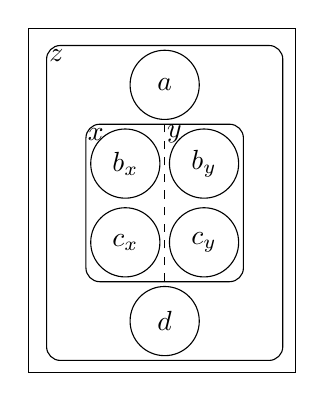
\begin{tikzpicture}[show background rectangle, scale=.5]  

\draw[rounded corners=5pt] (0,0) rectangle (6,8);  
\draw[rounded corners=5pt] (1,2) rectangle (5,6);  
\draw [dashed] (3,2) to[line to] (3,6);  

\node[state] (a) at (3,7)       {$a$};  
\node[state] (b_x) at (2,5)     {$b_x$};  
\node[state] (b_y) at (4,5)     {$b_y$};  
\node[state] (c_x) at (2,3)     {$c_x$};  
\node[state] (c_y) at (4,3)     {$c_y$};  
\node[state] (d) at (3,1)       {$d$};  
\draw (1.25,5.75) node {$x$};  
\draw (3.25,5.75) node {$y$};  
\draw (0.25,7.75) node {$z$};  

\end{tikzpicture}  

}  
% The only difference is here, where I have commented out an empty line.
\subfigure[After]  
{  

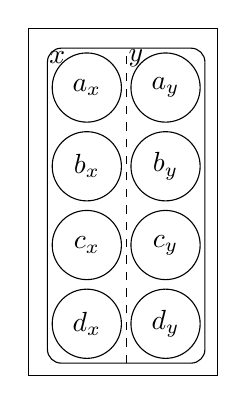
\begin{tikzpicture}[show background rectangle, scale = 0.5]  

\draw[rounded corners=5pt] (0,0) rectangle (4,8);  
\draw [dashed] (2,0) to[line to] (2,8);  

\node[state] (a_x) at (1,7)     {$a_x$};  
\node[state] (a_y) at (3,7)     {$a_y$};  
\node[state] (b_x) at (1,5)     {$b_x$};  
\node[state] (b_y) at (3,5)     {$b_y$};  
\node[state] (c_x) at (1,3)     {$c_x$};  
\node[state] (c_y) at (3,3)     {$c_y$};  
\node[state] (d_x) at (1,1)     {$d_x$};  
\node[state] (d_y) at (3,1)     {$d_y$};  
\draw (0.25,7.75) node {$x$};  
\draw (2.25,7.75) node {$y$};  
\end{tikzpicture}  

}

\caption{An example of the procedure}
\end{figure}
\end{document}